\chapter{Einleitung}

\section{Motivation}

WebAssembly \cite{WebAssemblyWebsite} ist eine neue Technologie mit dem Ziel, eine sprachunabhängige Plattform für das Web zu schaffen. Da nur JavaScript von Browsern unterstützt wird, ist man auf diese Sprache beschränkt. Früher konnte man auch Java-Applets mit Java entwickeln, die direkt im Browser ausgeführt werden konnten. Aktuelle Browserversionen unterstützen diese Technologie mittlerweile nicht mehr und Oracle stellt ebenfalls die Unterstützung ein \cite{OracleJavaSESupportRoadmap}.

Anders sieht es bei Sprachen wie beispielsweise TypeScript aus: Um diese im Browser ausführen zu können, muss der Quelltext zunächst mit einem Transpiler nach JavaScript übersetzt werden. Anschließend muss der resultierende JavaScript"=Quelltext vom Browser zur Laufzeit interpretiert werden \cite{TypeScript}.

WebAssembly verfolgt einen alternativen Ansatz, in dem eine Laufzeitumgebung in Form einer virtuellen Kellermaschine vom Browser zur Verfügung gestellt wird, so ähnlich wie früher die \emph{Java Virtual Machine} mit Java"=Applets. Über eine JavaScript"=Schnittstelle können zur Laufzeit Module geladen werden, die mit der virtuellen WebAssembly"=Maschine ausgeführt werden. Module müssen dafür in Form von WebAssembly"=Bytecode zur Verfügung stehen.

Ein geeigneter Compiler kann nun eine (beliebige) Programmiersprache in diesen Bytecode übersetzen. So ist ein Konvertieren des Quelltexts über einen Transpiler nicht mehr notwendig.

WebAssembly ist nicht als Alternative, sondern als Ergänzung zu JavaScript zu sehen. Ein Ziel ist, bestehenden Quelltext wiederverwenden zu können, auch wenn dieser in einer anderen Programmiersprache geschrieben wurde. Mit JavaScript werden die einzelnen Komponenten anschließend miteinander verbunden.

Damit dieses Ziel erreicht werden kann, müssen Compiler verschiedener Sprachen in der Lage sein, WebAssembly"=Bytecode zu erzeugen.

\section{Problemstellung}

Die Problemstellung für diese Masterarbeit lässt sich in folgende Fragen aufteilen:

\begin{enumerate}
	\item Was ist WebAssembly, welche Möglichkeiten bietet WebAssembly und welche Einschränkungen gibt es?
	\item Wie kann ein Compiler, der eine Programmiersprache nach WebAssembly übersetzt, implementiert und getestet werden?
	\item Wie werden typische Sprachkonstrukte einer Programmiersprache auf WebAssembly"=Befehle abgebildet?
	\item Wie wird die Schnittstelle zum Browser entworfen und auf welche Aspekte muss dabei geachtet werden?
\end{enumerate}

\section{Ziele}

Die Fragen der Problemstellung sollen auf auf Basis einer praktischen Implementierung beantwortet werden.

Ziel ist es, einen Compiler zu entwickeln, der MiniJava (eine Teilmenge von Java) nach WebAssembly übersetzt. Die Eingabe ist MiniJava"=Quelltext, die Ausgabe ein WebAssembly"=Modul samt Laufzeitsystem für JavaScript. Der gesamte Compiler wird in Kotlin entwickelt. Das Compiler"=Frontend (Scanner und Parser) wird mit ANTLR 4 generiert.

Schlussendlich soll es möglich sein, in MiniJava kleine, typische Web"=Anwendungen zu entwickeln.

Weiters wird eine minimale Standardbibliothek entworfen, diese stellt essentielle Schnittstellen für die Konsole und den DOM"=Zugriff zur Verfügung.

Es gibt bereits einige Technologien, die auf WebAssembly aufbauen. Auf drei ausgewählte wird in dieser Arbeit kurz eingangen:
\begin{itemize}
    \item Emscripten \cite{Emscripten} für C und C++,
    \item Rust \cite{RustWasmWebsite} und
    \item Blazor \cite{Blazor}.
\end{itemize}

Beim Einsatz von Emscripten und Rust ist im C/C++/Rust"=Quelltext ersichtlich, dass JavaScript oder WebAssembly im Hintergrund verwendet wird. Bei Emscripten sind das beispielsweise Einschlüsse von JavaScript"=Fragmenten oder bei Rust müssen spezielle Attribute eingefügt werden. Blazor ist ein Framework zum Entwickeln von Web"=Anwendungen und bietet somit eine Komplettlösung an. Hier kann bestehender C\#{}"=Quelltext unter gewissen Voraussetzungen wiederverwendet werden.

Mit MiniJava soll ein alternativer Ansatz versucht werden, eine (neue) Programmiersprache über WebAssembly in das Web zu bringen: MiniJava"=Quelltext soll im Unterschied zu Emscripten und Rust keine Hinweise darauf enthalten, dass der kompilierte Quelltext schlussendlich mit JavaScript und WebAssembly interagiert. Es soll mit MiniJava auch kein Framework aufgebaut werden wie bei Blazor. Weiters sollen Objekte in MiniJava 1:1 auf JavaScript"=Objekte abgebildet werden, dadurch soll beispielsweise direkter DOM"=Zugriff ermöglicht werden. Dieser Ansatz findet sich so in keiner der oben genannten drei Technologien. Schnittstellen zur Laufzeitumgebung werden in MiniJava über native Methoden umgesetzt. Dieses Sprachkonstrukt ist aus Java bekannt.

\section{Aufbau der Arbeit}

Die Arbeit ist in folgende, aufeinander aufbauende Kapitel gegliedert:
\begin{enumerate}
    \setcounter{enumi}{1}
    \item \emph{Technische Grundlagen:} Die Implementierung dieser Arbeit baut auf diversen Technologien auf. In diesem Kapitel werden die für diese Arbeit notwendigen Technologien beschrieben. Ein besonderer Fokus liegt hier auf WebAssembly und ANTLR, es wird aber auch auf diverse Hilfstechnologien eingegangen. Zum Schluss werden drei aktuelle Technologien im Detail betrachtet, die bereits WebAssembly"=Unterstützung anbieten.
    \item \emph{MiniJava und Anforderungen an den Compiler sowie das Laufzeitsystem:} In diesem Kapitel wird die Programmiersprache MiniJava vorgestellt. Dieses Kapitel ist als Art Anforderungskatalog für den Compiler und das Laufzeitsystem zu sehen.
    \item \emph{Codegenerierung für WebAssembly:} In diesem Kapitel wird gezeigt, wie aus MiniJava"=Quelltext ein WebAssembly"=Modul erzeugt wird. Dabei wird insbesondere gezeigt, wie die Sprachkonstrukte auf WebAssembly abgebildet werden. 
    \item \emph{Integration mit JavaScript:} Das erzeugte WebAssembly"=Modul benötigt zur Ausführung noch ein Laufzeitsystem, auf dieses wird in diesem Kapitel eingangen. Das Laufzeitsystem ist in JavaScript implementiert. Weiters wird vom Compiler auch JavaScript"=Quelltext generiert, um das Modul ausführen zu können.
    \item \emph{Testen des MiniJava"=Compilers und Integration in Gradle:} Um eine korrekte Funktion des Compilers zu gewährleisten, muss er getestet werden. Auf diesen Aspekt wird in diesem Kapitel im Detail eingangen. Weiters wird gezeigt, wie der Compiler in Gradle integriert werden kann, um ihn so in eigenen Projekten verwenden zu können. Diese Integration wird anhand einer Konsolenanwendung veranschaulicht.
    \item \emph{Demo"=Anwendungen im Browser:} In diesem Kapitel wird ein Fibonacci"=Rechner als Web"=Anwendung präsentiert, um die praktische Anwendung von MiniJava zu demonstrieren. Weiters wird hier kurz auf die Standardbibliothek für DOM"=Zugriffe eingangen.
\end{enumerate}

Zum Schluss werden die Ergebnisse der Arbeit zusammengefasst und es wird ein Ausblick auf mögliche Erweiterungen gegeben.

\pagebreak
\section{Architektur des Gesamtsystems}

Um zu Beginn einen Überblick zu geben, wird in Abbildung \ref{fig:architecture} die Architektur des Gesamtsystems dargestellt. Nachfolgend werden die wichtigsten Vorgänge beschrieben:

\begin{enumerate}
    \item Die Eingaben des Compilers sind MiniJava- und JavaScript"=Quelltexte. Die JavaScript"=Quelltexte enthalten die Implementierung nativer Methoden.
    \item Die MiniJava"=Quelltexte werden vom Scanner und Parser analysiert und in Syntaxbäume umgewandelt. Diese Syntaxbäume werden mit \emph{Visitors} und Codegeneratoren zu einem WebAssembly"=Modul (als Datenstruktur im Arbeitsspeicher) verarbeitet. Dabei werden ebenfalls Metainformationen über den MiniJava"=Quelltext gesammelt.
    \item Der Paketgenerator erzeugt aus dem Modul, den Meta"=Informationen und den JavaScript"=Quelltexten ein Paket. Ein Paket ist ein Verzeichnis mit einer definierten Struktur. Darin ist unter anderem das WebAssembly"=Modul als Datei enthalten.
    \item Das Laufzeitsystem lädt in der Laufzeitumgebung das Paket, dabei wird die WebAssembly"=API eingesetzt. Daraus entsteht ein lauffähiges Modul.
    \item Nun kann das Modul gestartet werden und Ausgaben auf der Konsole oder visuell im DOM erzeugen.
\end{enumerate}


\begin{figure}[]
    \centering
    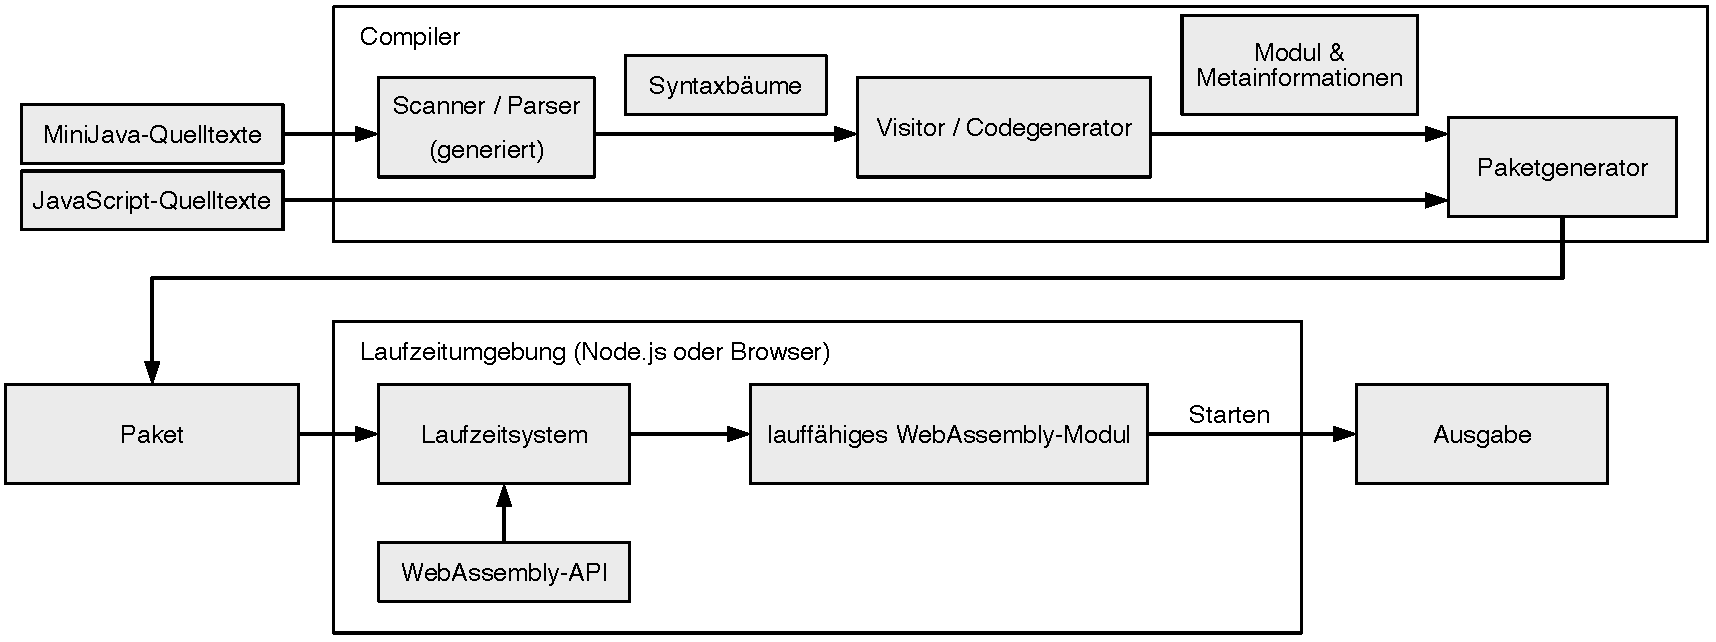
\includegraphics[width=\textwidth]{einleitung/architecture}
    \caption{Architektur des Gesamtsystems}
    \label{fig:architecture}
\end{figure}

\section{Verweis auf Quelltext}
Der Quelltext des gesamten Compilers und der Demo"=Beispiele steht auf GitHub zum Download zur Verfügung: \url{https://github.com/stefanschoeberl/MiniJava-Compiler}
